\documentclass[border=5pt]{standalone}
\usepackage{pgfplots}
\pgfplotsset{compat=1.18}
\usepackage{xcolor}

\definecolor{frankaBlue}{RGB}{31,119,180}
\definecolor{laikagoOrange}{RGB}{255,127,14}

\begin{document}
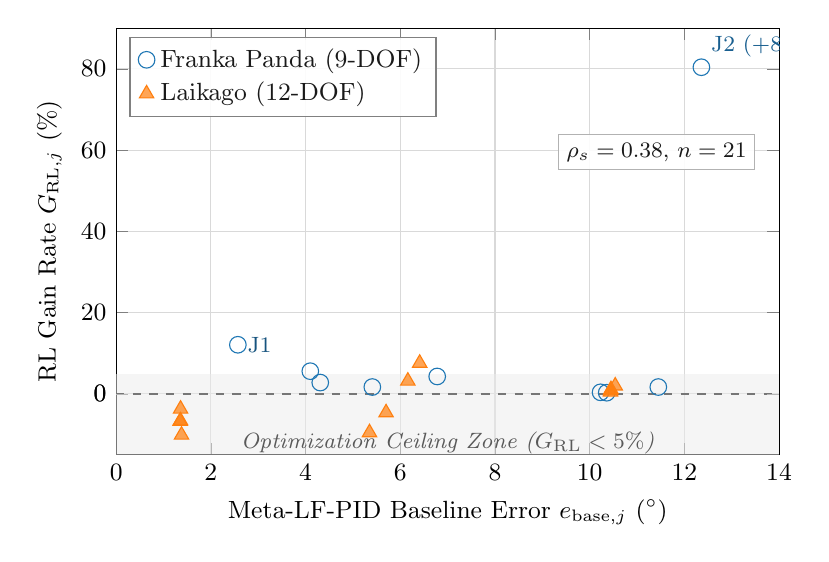
\begin{tikzpicture}
\begin{axis}[
    width=10cm,
    height=7cm,
    xlabel={Meta-LF-PID Baseline Error $e_{\mathrm{base},j}$ ($^\circ$)},
    ylabel={RL Gain Rate $G_{\mathrm{RL},j}$ (\%)},
    xmin=0, xmax=14,
    ymin=-15, ymax=90,
    grid=both,
    grid style={gray!30},
    legend style={at={(0.02,0.98)}, anchor=north west, font=\small,
                  draw=black!50, fill=white, fill opacity=0.9},
    legend cell align={left},
    tick label style={font=\small},
    label style={font=\small},
    % Reference line at G_RL = 0
    extra y ticks={0},
    extra y tick style={grid style={black, dashed, thick}},
]

% Franka Panda joints (blue circles)
\addplot[
    only marks,
    mark=o,
    mark size=3pt,
    color=frankaBlue,
    fill=frankaBlue,
    fill opacity=0.7,
] coordinates {
    (2.57, 12.1)
    (12.36, 80.4)
    (4.10, 5.6)
    (6.78, 4.3)
    (5.41, 1.7)
    (4.31, 2.8)
    (11.45, 1.7)
    (10.23, 0.4)
    (10.36, 0.3)
};
\addlegendentry{Franka Panda (9-DOF)}

% Laikago joints (orange triangles)
\addplot[
    only marks,
    mark=triangle*,
    mark size=3pt,
    color=laikagoOrange,
    fill=laikagoOrange,
    fill opacity=0.7,
] coordinates {
    (1.38, -10.1)
    (6.16, 3.2)
    (10.45, 1.1)
    (1.36, -6.6)
    (5.70, -4.6)
    (10.54, 2.0)
    (1.36, -3.7)
    (5.35, -9.5)
    (10.44, 0.8)
    (1.35, -6.7)
    (6.41, 7.6)
    (10.44, 0.5)
};
\addlegendentry{Laikago (12-DOF)}

% Annotate Franka J2 outlier
\node[above right, font=\footnotesize, color=frankaBlue!80!black] 
    at (axis cs:12.36, 80.4) {J2 (+80.4\%)};

% Annotate Franka J1
\node[right, font=\footnotesize, color=frankaBlue!70!black] 
    at (axis cs:2.57, 12.1) {J1};

% Shaded region for "ceiling zone" (low G_RL)
\fill[gray!15, opacity=0.5] (axis cs:0,-15) rectangle (axis cs:14,5);
\node[font=\footnotesize\itshape, color=gray!70!black] 
    at (axis cs:7, -12) {Optimization Ceiling Zone ($G_{\mathrm{RL}} < 5\%$)};

% Annotation: Spearman correlation
\node[font=\footnotesize, anchor=south east, fill=white, fill opacity=0.9, 
      draw=black!30, inner sep=3pt] 
    at (axis cs:13.5, 55) {$\rho_s = 0.38$, $n = 21$};

\end{axis}
\end{tikzpicture}
\end{document}
